\chapter{Autonomous Load Balancing in a Distributed Hash Table}
\label{chapter:auto-balance}




%http://michiel.buddingh.eu/distribution-of-hash-values

\section{Introduction}

%\subsection{2-4 sentences telling people what you will talk about in the paper}

%\subsection{What are DHTs}
Distributed Hash Tables (DHTs) are a class of well researched decentralized key-value storage systems.
DHTs are most frequently used to construct the overlays of P2P file-sharing systems, such as the incredibly popular BitTorrent \cite{bittorrent}.
DHTs have also been used in many unorthodox applications, such as machine learning \cite{liparameter} and, most relevant for our discussion, distributed computing \cite{chordreduce}.

Our previous research \cite{chordreduce} examined using a DHT as the organizing mechanism for a distributed platform.
This enabled us to create an exceptionally fault tolerant distributed computing platform that was easy to setup and could be run in a completely decentralized P2P environment.

% Copy into disseration start here
%\subsection{What is the significance of the hash function }
One of key components of a Distributed Hash Table is a cryptographic hash function, most commonly SHA1 \cite{sha1}.
Distributed Hash Tables rely on this cryptographic hash function to generate identifiers for data stored on the network.
The cryptographic hash of the filename or other identifier for the data is used as the location of the file or data in the network.
It can also be used to generate the identifiers for nodes in the network.

Ideally, inputing random numbers into a cryptographic hash function should produce a uniformly distributed output.
However, this is impossible in practice \cite{hash-outputs} \cite{thomsen2005cryptographic}.

In practice, that means given any DHT with files and nodes, there will be an inherent imbalance in the network.
Some nodes will end up with a lion's share of the keys, while other will have few responsibilities (Table \ref{tab:medianLoads}).


This makes it especially disheartening to try and ensure as even a load as possible.
We cannot rely on a centralized strategy to fix this imbalance, since that would violate the principles and objects behind creating a fully decentralized and distributed system.

Therefore, if we want to create strategies to act against the inequity of the load distribution, we need a strategy that individual nodes can act upon autonomously.
These strategies need to make decisions that a node can make at a local level, using only information about their own load and the topology they can see.


\subsection{Motivation}
The primary motivation for us is creating a new viable type of platform for distributed computing.
Most distributed computing paradigms, such as Hadoop \cite{hadoop}, assume that the computations occur in a centralized environments.
One enormous benefit is a centralized system has much greater control in ensuring load-balancing.

However, in an increasingly global world where computation is king and the Internet is increasingly an integral part of everyday life, single points of failure failures quickly become more and more risky.
Users expect their apps to work regardless of any power outage affecting an entire region.
Customers expect their services to still be provided regardless of any.
The next big quake affecting the the San Andreas fault line is a matter of when, not if.
Thus, centralized systems with single points of failure become a riskier option and decentralized, distributed systems the safer choice.


Our previous work in ChordReduce \cite{chordreduce} focused on creating a decentralized distributed computing framework based off of the Chord Distributed Hash Table (DHT) and MapReduce.
ChordReduce can be thought of a more generalized implementation of the concepts of MapReduce.
One of the advantages of ChordReduce can be used in either a traditional datacenter or P2P environment.\footnote{The other one being that new nodes could join during runtime and receive work from nodes doing computations.}
Chord (and all DHTs) have the qualities we desire for distributed computing: scalability, fault tolerance, and load-balancing.

Fault tolerance is of particular importance to DHTs, since their primary use case is P2P file-sharing, such as BitTorrent \cite{bittorrent}.
These systems experience high levels of churn-- disruptions to the network topology as a result of nodes entering and leaving the network.
ChordReduce had to have the same level of robustness against churn that Chord did, if not better.

During our experiments with ChordReduce, we found that high levels of churn actually made our computations run \textit{faster}.
We hypothesized that the churn was effectively load-balancing the network.

\subsection{Objectives}
This paper serves to prove our hypothesis that churn can load balance a Distributed Hash Table.
We also set out to show that we can use this in a highly controlled manner to greater effect.

We present three additional strategies that nodes can use to redistribute the workload in the network.
Each of these three strategies relies on nodes creating virtual nodes, and so that they are represented multiple times in the network.
The idea behind this is that a node with low work can create virtual nodes to seek out and acquire work from other nodes.

This tactic is the same one used in the Sybil \cite{sybil} attack, but limited in scope and performed for altruistic and beneficent reasons, rather than malicious ones.
Consequently, we'll call our virtual nodes in this scenario Sybils for clarity and brevity.
None of the strategies require a centralized organizer, merely a way for a node to check the amount of files or tasks it and its Sybils are responsible for.


We also want to show how distributed computing can be performed in a heterogeneous environment.
We want to see if our strategies result in similar speedups in both homogeneous and heterogeneous environments.
%\subsection{Summary}

%\section{Previous Work}
%
%
%ChordReduce \cite{chordreduce} is designed as a more abstract framework for MapReduce, able to run on any arbitrary distributed configuration.
%ChordReduce leverages the features of distributed hash tables to handle distributed file storage, fault tolerance, and lookup.
%We designed ChordReduce to ensure that no single node is a point of failure and that there is no need for any node to coordinate the efforts of other nodes during processing.

\section{How Work Is Distributed in DHTs: A Visual Guide}
%In this section, we display graphs to give a visual representation of how work is distributed in a Chord \cite{chord} network

As we have previously mentioned, many DHTs use a cryptographic hash function to choose keys for nodes and data.
However, no cryptographic hash function can uniformly distribute it's outputs across its range. 

\begin{table}
	\centering
	\caption{The median distribution of tasks (or files) among nodes.  We can see the standard deviation is fairly close to the expected mean workload ($\frac{tasks}{nodes}$). Each row is the average of 100 trials.}
	\begin{tabular}{r r r r}
		Nodes & Tasks & Median Workload & $\sigma$ \\ \hline
		1000 & 100000 & 69.410   &  137.27  \\
		1000 & 500000 & 346.570  &  499.169 \\
		1000 &1000000 & 692.300  &  996.982 \\
		
		5000 & 100000  & 13.810 & 20.477 \\ 
		5000 & 500000  & 69.280 & 100.344 \\ 
		5000 & 1000000 &138.360 & 200.564 \\ 
		
		10000 & 100000 & 7.000   &  10.492 \\
		10000 & 500000 & 34.550  &   50.366 \\
		10000 & 1000000& 69.180  &  100.319 \\
	\end{tabular}
	\label{tab:medianLoads}
\end{table}




\begin{figure}
	\centering
	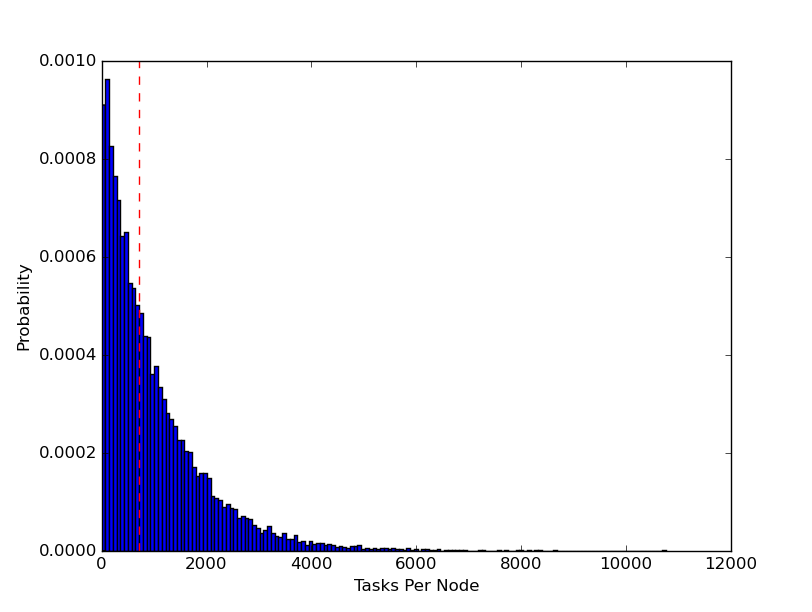
\includegraphics[width=0.7\linewidth]{figs/workloadDistribution}
	\caption[foo]{The probability distribution of workload in a DHT with 1000 nodes and 1,000,000 tasks or files.  The vertical dashed line designates the median.  Keys were generated by feeding random numbers into the SHA1 hash function \cite{sha1}, a favorite for many distributed hash tables.}
	\label{fig:workloadDistribution}
\end{figure}

An example Chord DHT.
Each node and task is given a 160-bit identifier \texttt{id} that is mapped to location $ (x,y) $ on the perimeter of the unit circle via the equations $ x = \sin\left( \frac{ 2 \pi \cdot id}{2^{160}} \right)$ and $ y = \cos\left( \frac{ 2 \pi \cdot id}{2^{160}} \right)$. 
Note that some of the nodes cluster right next to each other, while other nodes have a relatively long distance between each other along the perimeter.  
The most blatant example of this is the node located at approximately $(-0.67, 0.75)$, which would be responsible for all the tasks between that and the next node located counterclockwise.
That node and the node located at about $(-0.1, -1)$ are responsible for approximately half the tasks in the network.

\begin{figure}
\centering
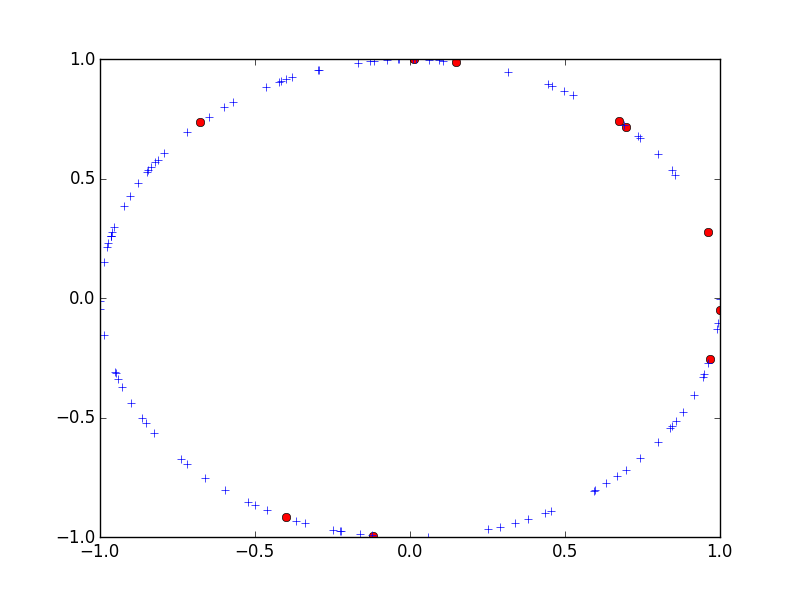
\includegraphics[width=0.7\linewidth]{figs/exampleChordDistribution}
\caption[Distribution of Nodes and Tasks in a Chiord DHT]{A visual example of data and nodes in a Chord DHT with 10 nodes (represented by red circles) and 100 tasks (blue pluses). Nodes are responsible for all the tasks that fall along the perimeter between themselves and their predecessor, which is the closest node counterclockwise.}
\label{fig:exampleChordDistribution}
\end{figure}



\section{Simulation}
\label{sec:auto-simulation}

%We simulate an UrDHT Voronoi based-network in multiple dimensions. \footnote{UrDHT in one dimension is a Chord ring with the definition of responsibility changed to a node being responsible to all data closest to it. A 2-dimensional network will emulate the performance of CAN.}


We will be simulating our strategies on a Chord distributed hash table \cite{chord}, although it is fairly straightforward to implement our strategies for other, more complex DHTs.
Nodes in a Chord ring are given an ID, drawn from a cryptographic hash function, typically SHA1 \cite{sha1}.
Any data in the network is given a key in a similar manner.
Nodes are responsible for all the keys between their predecessor's ID and their own.

We assume that the network starts our experiments stable and the data necessary already present on the nodes and backed-up.
The following analysis and simulation relies on an important assumption about DHT behavior often assumed but not necessarily implemented.


We assume that nodes are active and aggressive in creating and monitoring the backups and the data they are responsible for.
%Specifically, we will assume it takes  $T_{detect}$ time for a node to detect a change in their responsibility or to detect a new node to hand a backup to and that this check is performed regularly. 
We have demonstrated the effectiveness and viability of implementing an active backup strategy in other work \cite{chordreduce} \cite{urdht}.
As previously mentioned, we also assume nodes have the ability to examine the amount of work they have and know how many tasks or pieces of data exist for a particular job.

Another assumption is that nodes do not have control in choosing their IDs from the range of hash values.
This means that nodes cannot automatically change their spacing to ensure they are all evenly spread out across the network.
Likewise, nodes cannot create necessarily create Sybils exactly where they would like, but would have to search for an appropriate ID in between two other nodes.
We discussed this process in previous work and showed that it is extremely quick for a node to do so \cite{sybil-analysis}.



%Smaller chunking results in more files spread throughout the network and a greater chance of the data being evenly spread across the network 


%The chances of a critical failure happening within a time interval $ T $ is the chances of some chain or cluster of nodes responsible for a single record dying within $ T $:
%
%$$r^{s}$$
%
%Where $ r $ is the failure rate over that time interval and $s$ is the number nodes storing that record, either as a primary system, or a backup.
%Incidentally, this time interval $T = T_{detect} + T_{transfer} $
%


\subsection{The Parameters}

Our simulations relied on a great number of parameters and variables.
We present each of them below.

\subsubsection{Constants and Terminology}

First, we'll define informally define the vocabulary we use to discuss our simulations.

\begin{description}
	\item [Tick] In a simulation, normal measurements of time such as a second are completely arbitrary.  
	We will be using an abstract \textit{tick} to measure time.  
	We consider the tick the amount of time it takes a node to complete one task (or more depending on our variables, see below) and perform the appropriate maintenance to keep the network consistent and healthy.\footnote{If we need to be more concrete, define a tick as a New York Second, which is ``the period of time between the traffic lights turning green and the cab behind you honking.''\\-- Terry Pratchett}
	\item [Maintenance] We assume nodes use the active, aggressive strategy from ChordReduce and UrDHT \cite{chordreduce} \cite{urdht}.
	Every maintenance cycle, each node checks and updates its list of neighbors (successors and predecessors in Chord) and responds appropriately. 
	We assume that a tick is enough time to accomplish at least one maintenance cycle.
	\item[Task] We measure the size of a distributed computing job in tasks.
	Each task has a key that corresponds to the key of a file or chunk of a file stored on the network.
	We assume that it takes a tick for a node to consume at least one task.
	\item [IDs and Keys] 
	We will be using SHA-1 \cite{sha1}, a 160-bit hash function, to generate node IDs and keys for tasks.  
	We assume each task's key corresponds to some piece of data with the same key, a scheme we used in  our previous work on ChordReduce \cite{chordreduce}.
\end{description}

\subsubsection{Experimental Variables}
We tested a number of strategies and variables that could affect each strategy.
While we believed the overall strategy would result in largest differences in runtime, we wanted to see what effects, if any, each of the variables would have on a particular strategy.

\begin{description}
	\item [Strategy] We use several different strategies, each discussed in Section \ref{sec:strategies}: churn, random injection, neighbor injection, and invitation.
	Each of these strategies differs in how nodes attempt  to autonomous balance the workload of the network.
	None of the strategies require centralized organization.
	\item [Homogeneity]  This variable controls whether the network is homogeneous or not.
	In a homogeneous network, each node has the same strength, which dictates how much work is consumed per a tick and how many Sybils it can create.
	In a heterogeneous network, each node has a strength chosen uniformly at random from 1 to \texttt{maxSybils}.
	\item [Work Measurement] This variable dictates how much work is consumed in a tick.
	Each node can either consume a single task per a tick or their strength's worth of tasks per a tick.
	\item [Network Size]  How many nodes start in the network.  
	We assume that this can grow during the experiment, either via churn or by creating Sybils.
	We discuss how this works in Sections \ref{sec:strat-churn} and \ref{sec:strat-randomInject}.
	\item [Number of Tasks] We measure the size of of a job in tasks.
	This number is typically a few orders of magnitude greater than the network size.
	\item [Churn Rate] The churn rate is a float between 0 and 1.
	This represents both the chance each individual node has of leaving (or joining) the network each tick.
	It also corresponded to the fraction of nodes we expect to leave the network each tick.
	Churn can be self induced or a result of actual turbulence in the network.
	Like most analyses of churn \cite{marozzo2012p2p}, we assume churn is constant throughout the experiment and that the joining and leaving rate are equal.
	\item [Max Sybils] \texttt{maxSybils} is the maximum number of Sybils a node can have at once.
	\item [Sybil Threshold] The \texttt{sybilThreshold} dictates the number of tasks a node must have before it can create a Sybil.
	\item [Successors] The number of successors each node keeps track of.  
	Nodes also keep track of the same number of predecessors.
	
\end{description}

We also considered using a variable noted as the \texttt{AdaptationRate}, which was the interval at which nodes decided whether or not to create a Sybil.
Preliminary experiments showed \texttt{AdaptationRate} to have a minimal effect on the runtime, so it was removed.

\subsubsection{Outputs}
The most important output was the number of ticks it took for the experiment to complete.
We compared this runtime to the what we call the ``ideal runtime,'' which is our expected runtime if the every node in the network was given an equal number of tasks and performed them without any churn or creating any Sybils.
For example, consider a network with 1,000 nodes and 100,000 tasks, where each node consumes a single task each tick. 
This network has an ideal runtime of 100 ticks ($ \frac{100000}{1000} = 100$).\footnote{The ideal runtime also happens to be the average number of tasks per node. An interesting, but mathematically unsurprising, coincidence with a few consequences for our data collection.} 

We used these to calculate a ``runtime factor,'' the ratio of the experimental runtime compared to the ideal runtime.
For example, in the network from our previous example took 852 ticks to finish, its factor is 8.52.
We prefer to use this runtime factor for comparisons since it allows us to compare networks of different compositions, task assignments, and other variables.

We also collected data on the average work per tick and statistical information about how the tasks are distributed throughout the network.
We additionally performed detailed observations of how the workload is  distributed and redistributed throughout the network during the first 50 ticks.

\section{Strategies}
\label{sec:strategies}

For our analysis, we examined four different strategies for nodes to perform autonomous load balancing.
We first show the effects of churn on the speed of a distributed computation.
We then look a three different strategies for in which nodes take a more tactical approach for creating churn and affecting the runtime.

Specifically, nodes perform a limited and controlled Sybil attack \cite{sybil} on their own network in an effort to acquire work with their virtual nodes.
Our strategies dictate when and where these Sybil nodes are created.

We discuss the effectiveness of each of the strategies and present the results of our simulations in Section \ref{sec:autonomous-results}.



\subsection{Induced Churn}
\label{sec:strat-churn}
Our first strategy, \textit{Induced Churn}, relies solely on churn to perform load balancing.
This churn can either be a product of normal network activity or self-induced.\footnote{All distributed systems experience churn, even if only as hardware failures.}
By self-induced churn, we mean that each node generates a random floating point number between 0 and 1.
If the number is $\leq churnRate$, the node shuts down and leaves the network and gets added to the pool of nodes waiting to join.

Similarly, we have a pool of waiting nodes that begins the same initial size as the network.
When they generate an appropriate random number, they join the network and leave the waiting pool.
We assume that nodes enter and leave the network at the same rate.
Because the initial size of the network and the pool of waiting nodes is the same and nodes move between one another at the same random rate, the size of either does not fluctuate wildly.

As we have previously discussed, nodes in our network model actively back up their data and tasks to the a number of successors in case of failure.
In addition, when a node joins, it acquires all the work it is responsible for.
While this model is rarely implemented for DHTs, it is discussed \cite{kademlia} and often assumed to be the way DHTs operate. 
We have implemented it in ChordReduce\cite{chordreduce} and UrDHT\cite{urdht} and demonstrated that the network is capable from recovering from quite catastrophic failures and handling ludicrous amounts of churn.

The consequences of this are that a node suddenly dying is of minimal impact to the network.
This is because a node's successor will quickly detect the loss of the node and know to be responsible for the node's work.
Conversely, a node joining in this model can be a potential boon to the network by joining a portion of the network with a lot of tasks and immediately acquiring work.

This strategy acts as a baseline with which to compare the other strategies, as it is no more than a overcomplicated way of turning machines off and on again. 
All strategies below are attempts to do better than random chance.
However, this strategy also serves to confirm the speedup phenomenon we observed in our previous work on a distributed, decentralized MapReduce framework \cite{chordreduce}.

\subsection{Random Injection}
\label{sec:strat-randomInject}
Our second strategy we dubbed \textit{Random Injection}.
In this strategy, once a node's workload was at or below the \texttt{sybilThreshold}, the node would attempt to acquire more work by creating a Sybil node at a random address.

A node compares its workload to the \texttt{sybilThreshold} and decides whether or not to make a Sybil.
This check occurs every 5 ticks.
A node cam also have multiple Sybils, up to \texttt{maxSybils} in a homogeneous network or the node's \texttt{strength} in a heterogeneous network.\footnote{No benefit was shown by increasing \texttt{maxSybils} beyond 10.}
If a node has at least one Sybil, but no work, it has its Sybils quit the network.
We limit each node to creating a single Sybil during this decision to avoid overwhelming the network.

%As we discuss in Section \ref{sec:autonomous-results}, this strategy is surprisingly effective and comes close to ideal runtimes.



\subsection{Neighbor Injection}
\label{sec:strat-neighbor}
\textit{Neighbor Injection} also creates Sybils, but in this case, nodes act on a more restricted range in an attempt to limit the network traffic.
Nodes with \texttt{sybilThreshold} or less tasks attempt to acquire more work by placing a Sybil among it's successors.
Specifically, it looks for the biggest range among it's successors and creates a Sybil in that range.

This range strategy of finding the largest range and injecting assumes that the node with the largest range of responsibility will have been allocated the most work.
This is a sensible assumption since the larger the range of a node's responsibility, the more \textit{potential} tasks it can receive. 
We compare this estimation strategy to actually querying the neighbor and asking how many tasks they have.
An estimation, if accurate, would be preferable to querying the nodes as an estimation can be done without any communication with the successor nodes.

To avoid constant spamming of a range, once a node creates a Sybil, but does not acquire work, it may be advisable to mark that range as invalid for Sybil nodes so nodes don't keep trying the same range repeatedly. 


\subsection{Invitation}
The \textit{Invitation} strategy is the reverse of the Sybil injection strategies.
In  this strategy, nodes with a higher than desired level of work announces it needs help to its predecessors.
The predecessor with least amount of tasks less than or equal to the \texttt{sybilThreshold} creates a Sybil to acquire work from the node.
It is possible for an invitation to get more work to be refused by anyone if no  predecessor is at the \texttt{sybilThreshold} or each predecessor has too many Sybils.
Nodes determine whether or not they are overburdened using the \texttt{sybilThreshold}.



\section{Results Of Experiments}
\label{sec:autonomous-results}

We now briefly summarize the results of our simulation before discussing each more in depth below.
First, we confirmed that churn, even at low levels, can speed up the execution of a distributed computation by dynamically load balancing the network.
However, our best strategy was random injection, which managed to have a runtime factor which approached close to 1.

All examples are compared against against a baseline network of the same size and initial configuration of nodes. 
The only difference is that the baseline never uses a strategy or experiences any churn.

All the raw data can be found online \cite{simulation-data}.
Files are sorted by the strategy used, the network size,  and number of tasks and include the both the results of each individual run and the averages of each 100 trials for a particular set of variables.
Each trial is linked with a seed for the pseudorandom number generator and can be fully reproduced.


\subsection{Churn}

Our results confirmed our hypothesis from ChordReduce \cite{chordreduce}.
Churn has a profound and significant impact on the network's computation, and this effect is more pronounced with higher rates of churn.
Our results in Table \ref{tab:ChurnRuntimesHomogenious} show the effects of churn in networks of varying sizes and loads on the runtime factor.


\begin{table}[h]
	\tiny
	\centering
	\caption[Churn Runtimes in a homogenious network]{Runtime factor of networks of varying sizes and number of tasks, each using the Churn strategy to load-balance.  Each result is the average of 100 trials. The networks are homogeneous and each node consumes one task per tick.  A runtime of 1 is the ideal and target.}
	\begin{tabular}{|r || r | r | r | r | r |}
		\hline
		Churn Rate & $ 10^{3}$ nodes, $ 10^{5}$ tasks & $ 10^{3}$ nodes, $ 10^{6}$ tasks & $ 100$ nodes, $ 10^{4}$ tasks & $ 100$ nodes, $ 10^{5}$ tasks &$ 100$ nodes, $ 10^{6}$ tasks \\ \hline
		0      & 7.476   &  7.467 &  5.043& 5.022 &5.016 \\\hline
		0.0001 & 7.122   &  5.732 &  4.934& 4.362&3.077 \\\hline
		0.001  & 6.047   &  3.674 &  4.391& 3.019  &1.863\\\hline
		0.01  &  3.721   &  2.104 &  3.076& 1.873 &1.309\\\hline
		
	\end{tabular}
	\label{tab:ChurnRuntimesHomogenious}
\end{table}

We see that for each network size and load, even small amounts of churn have a noticeable impact on churn.
The magnitude of churn's effect varies based on the size of the network and the number of tasks.
In networks where there are fewer nodes, we see the base runtime factor is smaller.
The gains from churn are most strongly related the number of tasks the network has, with the more tasks there are, the greater the gains of churn.
A network 100 nodes and 1 million tasks, on average, has a runtime factor only 30\% higher than ideal when churn is 0.01 per tick.
The runtime for heterogeneous versus homogeneous networks had no significant differences.


We ran additional experiments on rates of churn for a 1000 node network and 100,000 tasks, in order to give a fuller picture of the effects of churn.
We tested this network with a wider variety of churn rates.
The results of this are shown on Figure \ref{fig:churnVsTime}, which plots the runtime of the distributed computation against the level of churn in the network.


\begin{figure}[h]
	\centering
	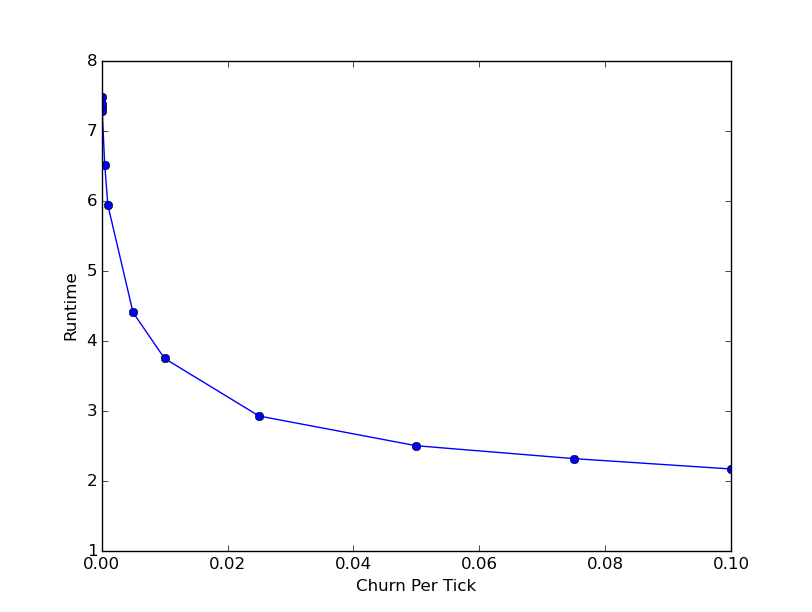
\includegraphics[width=0.7\linewidth]{figs/churnVsTime}
	\caption[Churn vs Runtime factor]{This graph shows the effect churn has on runtime in a distributed computation.
		Runtime is measured as how many times slower the computation runs than an ideal computation, where each node receives an equal number of tasks.
		The lower the runtime factor, the closer it is to an ideal of 1.
		Neither the homogeneity of the network nor work measurement had a significant effect on the runtime.}
	\label{fig:churnVsTime}
\end{figure}

We note the significantly diminishing returns that occur after a churn rate of 0.01.
One facet not captured by our simulations, but is significant, is the rising maintenance costs after that point.
The makes any amount of churn after a certain point prohibitively expensive.
What this point is requires implementation on a real network.

This speedup is reflected in the average number of tasks consumed in a tick, shown in Figure \ref{fig:churnVsWork}.
In a stable network with no churn, we would expect a good portion of the network to end up with little work, which is quickly consumed.
These nodes must then idle, waiting for the few nodes which received a large number of tasks to finish.
When there is churn, however, nodes have a chance of joining the network and acquiring more work, thus making it possible for more work to be done per a tick.
The higher the rate of churn, the more this happens.

\begin{figure}
\centering
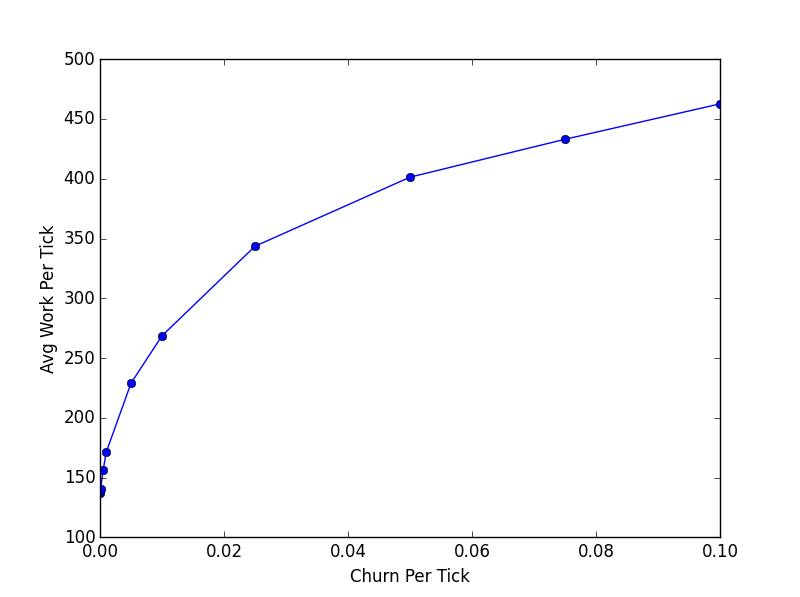
\includegraphics[width=0.7\linewidth]{figs/churnVsWork}
\caption[Churn vs average work per tick]{With more and more churn in the network, new nodes have a higher chance of joining the network and acquiring work from overloaded nodes.  This results in more average work being done each tick, as there are less nodes simply idling.}
\label{fig:churnVsWork}
\end{figure}



A more detailed view of how this happens is shown in Figures \ref{fig:churnStableHist0}, \ref{fig:churnStableHist5}, and \ref{fig:churnStableHist35}.
These figures show histograms of workload distribution for two networks at different ticks.
One network uses 0.01 churn per tick to autonomously load balance the workload, the other uses no strategy at all.

Both networks \footnote{Indeed, all networks we do this assessment for start with the same initial configuration} start with the 1000 nodes and 100,000 tasks distributed identically throughout the network. 
Figure \ref{fig:churnStableHist0} shows the distribution of the workload for this initial configuration.

As the network begins to work, we see the distributions diverge from one another.
Figure \ref{fig:churnStableHist5} shows that after merely 5 ticks, the network using the churn strategy has noticeably fewer nodes that have smaller workloads.
We also see more nodes with greater workloads.
The effect becomes even more pronounced after 35 ticks, shown in Figure \ref{fig:churnStableHist35}, where more have had a chance to finish their work and more churn has had the opportunity to occur.

\begin{figure}
\centering
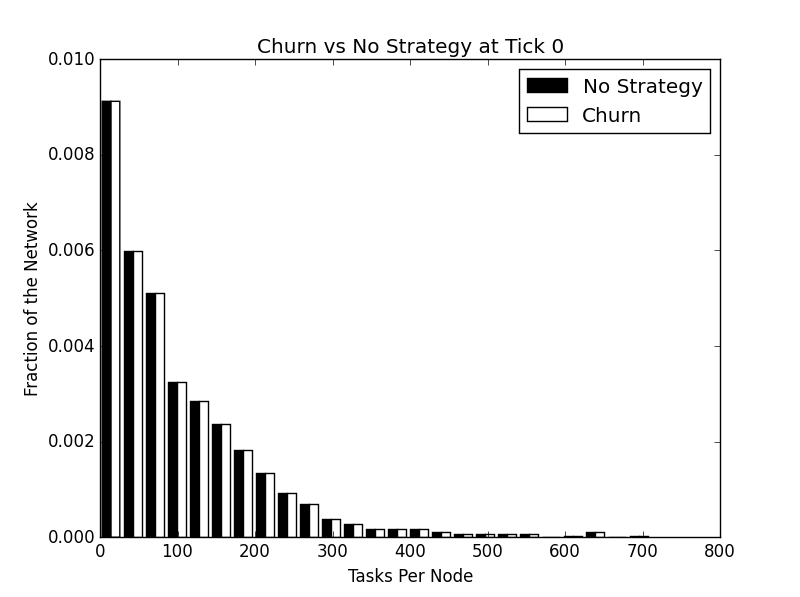
\includegraphics[width=0.7\linewidth]{figs/ChurnStableHist0}
\caption[Workload for churn at tick 0]{The initial distribution of the workload in both networks.  As both networks start with same initial configuration, the distribution is currently identical.  This greatly resembles the distribution we saw in Figure \ref{fig:workloadDistribution}.}

\label{fig:churnStableHist0}
\end{figure}


\begin{figure}
\centering
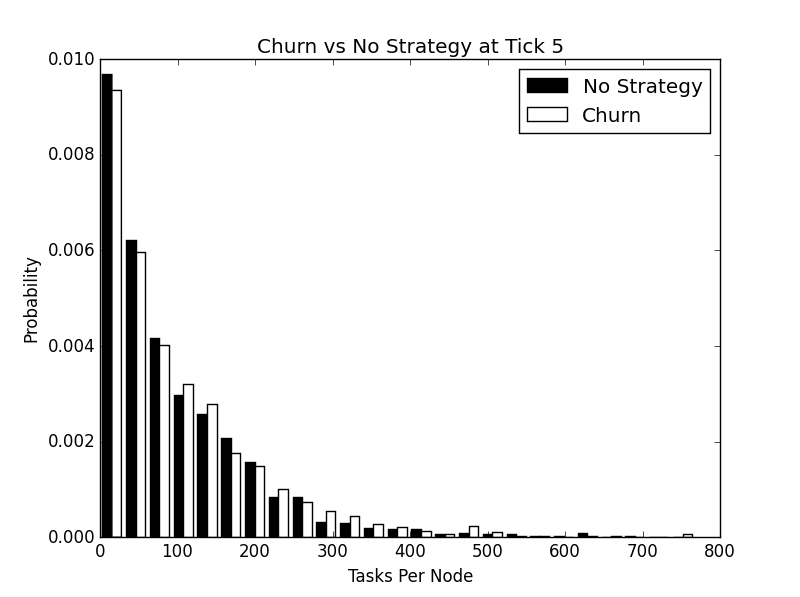
\includegraphics[width=0.7\linewidth]{figs/ChurnStableHist5}
\caption[Workload for churn at tick 5]{This is the distribution of the workloads at the beginning of tick 5.  We can see the network using 0.01 churn has fewer nodes with less work and more nodes with a greater workload.}

\label{fig:churnStableHist5}
\end{figure}



\begin{figure}
	\centering
	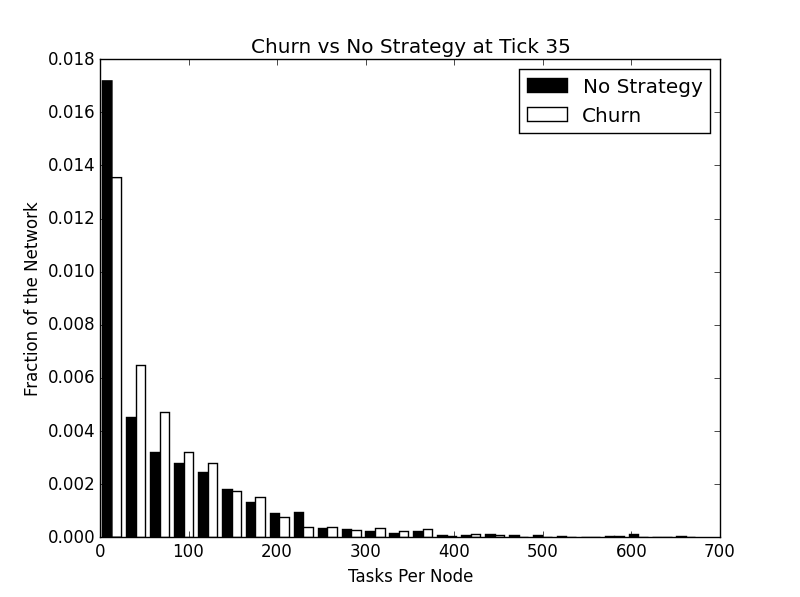
\includegraphics[width=0.7\linewidth]{figs/ChurnStableHist35}
	\caption[Workload for churn at tick 35]{After 35 ticks, the effects of churn on the workload distribution become more pronounced.  More nodes have consumed all their tasks and are simply idling, but significantly less in the network using churn.}
	\label{fig:churnStableHist35}
\end{figure}

\subsection{Random Injection}

The goal behind the churn strategy was to effectively have nodes join in the proper place with random insertions.
However, churn relies on two factors that are completely random.
The network nor it's members have any control over when node joins happen or where these joins occur.
In addition, churn removes nodes, which can be detrimental to the network.

The random injection strategy removes some of the randomization that the churn churn strategy deals with, namely \textit{when} new nodes join, albeit not where.
As we discussed earlier, random injection does this by means of the Sybil Attack \cite{sybil}, with nodes creating virtual Sybil nodes when they are underutilized.

We found that the strategy of having under-utilized nodes randomly create Sybil nodes works phenomenally well, approaching very close to the ideal time.
Figures \ref{fig:randomStableHist5} and \ref{fig:churnStableHist35} compare two networks with identical starting configurations as the network preforms the computations.\footnote{We omit a figure comparing the two networks at tick 0, since it identical to Figure \ref{fig:churnStableHist0}.}
These networks have 1000 nodes and 100,000 tasks.  
The network using random injection.


\begin{figure}
	\centering
	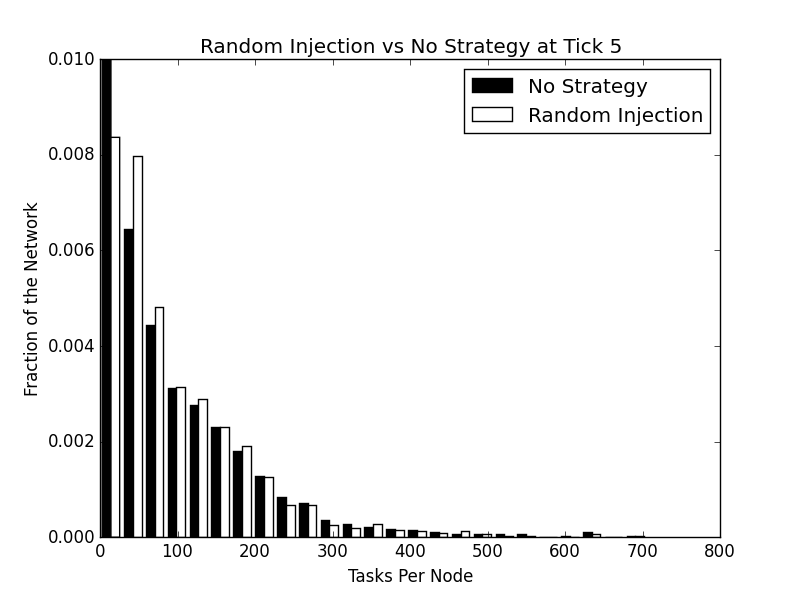
\includegraphics[width=0.7\linewidth]{figs/randomStableHist5}
	\caption[Random injection vs no strategy after 5 ticks.]{The networks after 5 ticks.  The network using random injection has significantly less underutilized nodes, even after only 5 ticks.}
	\label{fig:randomStableHist5}
\end{figure}


\begin{figure}
	\centering
	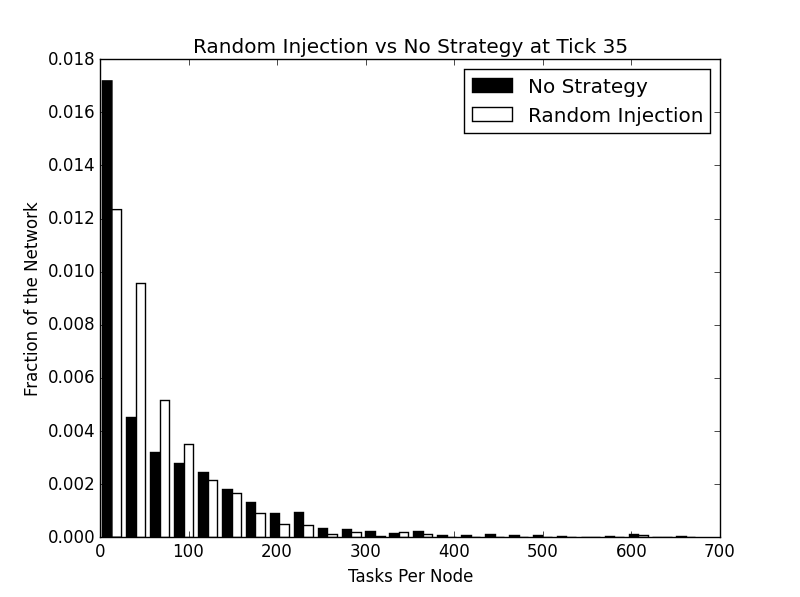
\includegraphics[width=0.7\linewidth]{figs/randomStableHist35}
	\caption[Random injection vs no strategy after 35 ticks.]{The networks after 35 ticks.  The network using random injection has significantly less underutilized nodes and substantially more notes with some or lots of work.}
	\label{fig:randomStableHist35}
\end{figure}


We can see in Figure \ref{fig:randomStableHist5}, the results of a single load balancing operation.
Each node has checked its workload, and if it was too low, created a single Sybil.
If we compare this to Figure \ref{fig:churnStableHist0}, we see that this single operation has a better workload distribution than what we had started with and is substantially better than using no strategy.

We can see these effects become even more pronounced at tick 35 (Figure \ref{fig:randomStableHist35}), where seven load balancing operations have taken place.
The network using random injection has many fewer nodes with little or no work and many more nodes with some work.
Furthermore, we see a huge difference between the effectiveness of random injection versus churn (Figure \ref{fig:churnInjectionHist35}).

\begin{figure}
	\centering
	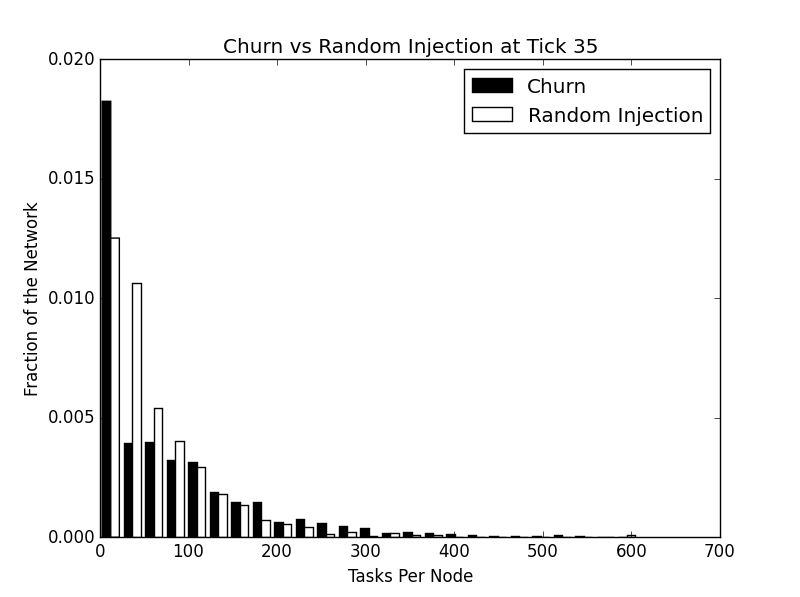
\includegraphics[width=0.7\linewidth]{figs/churnInjectionHist35}
	\caption[Churn vs Random Injection after 35 ticks.]{The networks after 35 ticks.  The network using random injection load-balances significantly better than the network using Churn.}
	\label{fig:churnInjectionHist35}
\end{figure}

We found that a homogeneous, 1000 node 100,000 task network, where each node consumed a single task each tick would never have an average runtime factor great than 1.7 and the average runtime was as fast as 1.36.
In the same network with 1,000,000 tasks, these runtimes were 1.25 and 1.12 respectively.
On average, the 1,000,000 task network had a runtime factor 0.82 less than the 100,000 task network.
This huge jump is the result of how the network is impacted by heterogeneous nodes, explained further below.

Overall we found that networks with the same ratio of tasks to nodes would have relatively the same runtimes, but the smaller network would run slightly faster.
For example, we compared two networks with 100 tasks per a node: a network with 100 nodes and 100,000 tasks and one with 1,000 nodes and 1,000,000 tasks.
The smaller network had, on average, a mean runtime factor 0.086 less.

Heterogeneous networks also saw significantly better performance (Figure \ref{fig:randomStableHistHetero35}), but the gains were not as great as in homogeneous networks.

\begin{figure}
\centering
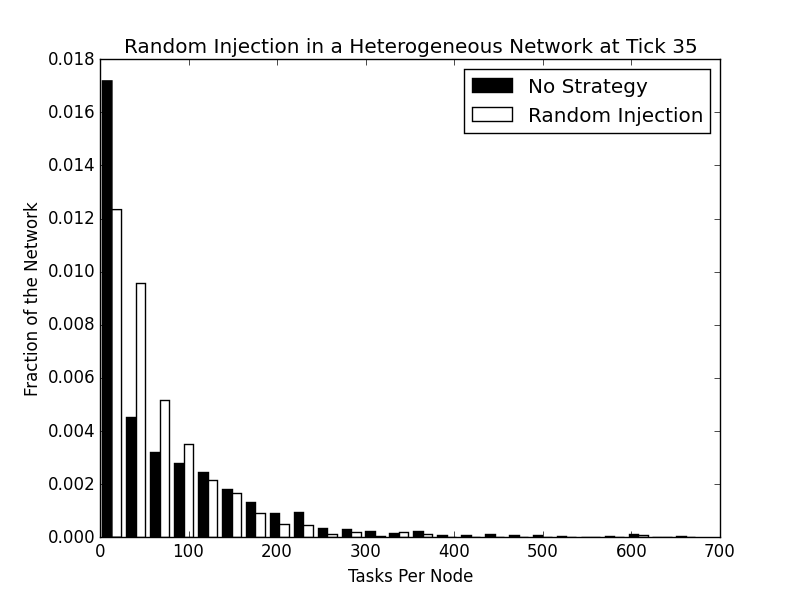
\includegraphics[width=0.7\linewidth]{figs/randomStableHistHetero35}
\caption[Random injection in a Heterogenous Network]{The workload distribution of heterogenous networks after 35 ticks}
\label{fig:randomStableHistHetero35}
\end{figure}



\subsubsection{The Effects of Other Variables}
However, the larger ratio networks handled heterogeneity much better, with the worst heterogeneous run time being 1.955, compared to 4.052 on  the smaller ratio networks

Sybil Threshold had an effect in homogeneous networks but no effect in heterogeneous networks.
In 1k100k and 1h1k experiment, a homogeneous network where each node completed one task per a tick, this amounted to an reduction of at least 0.1 runtime factor.
The effect was more pronounced when networks could complete a number of tasks equal to their strength each tick, reducing the runtime factor by at least 0.2.



However, we saw no corresponding speedup in the 1k1m and 1h100k networks.
We also found the \texttt{sybilThreshold} had no discernible effect on the runtime of heterogeneous networks.
This suggests the effect of a particular \texttt{sybilThreshold} is tied to the ratio of nodes to tasks and that the larger the ratio, the less room there is to improve.


Churn had no positive impact on the runtime factor and at higher levels could begin having an extremely minor impact when churn is at 0.01 per tick, increasing the average runtime factor by approximately 0.06 
\subsection{Neighbor Injection}


On average, the strategy of probing each of the neighbors before inserting, rather than estimating 
\subsection{Invitation}

In invitation, churn losses can be greatly detrimental.

\section{Future Work}

As mentioned in Section \ref{sec:auto-simulation}, we made the assumption that nodes cannot choose their own ID and must rely on the strategies described in Chapter \ref{chapter:sybil}  \cite{sybil-analysis} for creating a Sybil with the appropriate ID.
However, if this assumption was removed, this presents even more strategies for nodes to autonomously load-balance.